%!TEX root = ../../thesis.tex


\subsection{Relative differential amplitude}
\label{subsec:relative_differential_amplitue}
Further investigation was performed into the differential subtraction under small \(\Delta {RV}\).
This is done by exploring the amplitude of the differential against a variation in {RV}.
Simulations were performed creating a differential spectra for a range of \(\Delta {RV}\)s between \(\pm10\)\kmps{} using the same {PHOENIX-ACES} spectra for the companion of {HD\,30501} (\Teff{}=2500\K{}, \Logg{}=5.0, \feh{}=0.0) convolved to \(\R=50\,000\).
These simulations were focus on the wavelength range 2110--2123\nm{}, corresponding to detector \#1 of the {CRIRES} observations.
The differential spectra was created for each by taking the synthetic spectrum for the companion, Doppler shifting a copy of the spectrum and subtracting it from the original.
At each {RV} step the maximum absolute differential amplitude (peak to peak) of the simulated differential spectrum observed was recorded.
Again these simulations are performed assuming perfect telluric correction and removal of the host star by only considering the spectrum of the companion alone.

The result of this simulation is shown in \cref{fig:diff_amp}.
As this absolute amplitude is specific to the lines present in the analysed wavelength range, the values were normalized by the median amplitude value outside of the line {\fwhm} (dashed vertical lines), between \(\pm(7-10)\)\kmps{}, to give a relative differential amplitude, independent from the depth of a specific line.
Differential subtraction simulations we also performed using a spectrum made up of a single Gaussian or Lorentzian line; these are shown in \cref{fig:diff_amp} as the orange dashed and green dash-dotted lines respectively.
The spectral profile shape of the differential for the Gaussian line was also checked for consistency with the analytical form of the differential spectra from~\citet[][Equation~A.1]{ferluga_separating_1997} (included above as \cref{eqn:sprofile_gaussain}).

\cref{fig:diff_amp} shows that with a \(\Delta {RV}\) of zero between companion spectra the spectral lines of the companion completely cancel each other out, resulting in zero amplitude.
As the {RV} separation increases in either direction, the individual lines stop completely cancelling begin as they begin to separate.
A maximum differential amplitude is achieved when the individual lines are fully separated.
The shape/width of the differential spectral lobes~\citet[e.g.][eqn.~A.1]{ferluga_separating_1997} was not considered, but this could also have been measured.

At simulated separations beyond 10\kmps{} the neighbouring spectral lines begin to strongly interfere, leading to a variable (quasi-sinusoidal) relative amplitude, although this is not shown here.
The shape of the relative amplitude becomes complicated due to the line interaction and because the \(\Delta {RV}\) for all observations fall well short of this region it was not investigated further.
It is suspected that the interaction of neighbouring lines is one possible cause for the difference in the relative differential amplitude between the single theoretical line profiles and synthetic spectrum between 2 and 6\kmps{}.

The vertical dotted lines indicate the line \(\rm {\fwhm} = \lambda /\R=v /c\) with a velocity of 6\kmps{} at 2\um{} with \R=50\,000, showing that the amplitude is almost maximum when the lines are separated beyond their line width.
The two solid vertical lines in \cref{fig:diff_amp} indicate the \(\Delta \textrm{RV}\)=1.41\kmps{} separation calculated for our best target, {HD\,30501} from \cref{tab:estimated_rv}, given known orbital parameters and the observation times.
This shows that our differentials have severely reduced amplitude, \(<20\%\) relative to well separated individual lines.
As the companion spectra are already faint and in combination with a host star at >1\% flux ratio the >80\% extra reduction in signal amplitude makes this detection impossible with these observations.

\begin{figure}
    \centering
    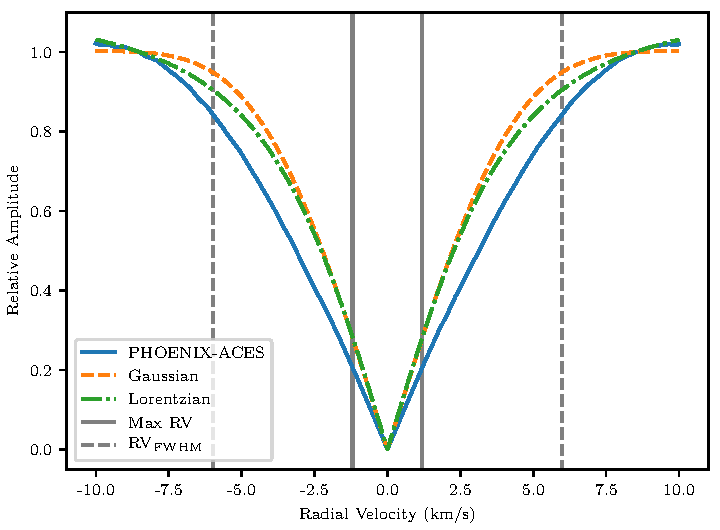
\includegraphics[width=0.8\textwidth]{figures/direct-recovery/rv_diff_final.pdf}
    \caption[Simulated relative amplitude of differntial spectrum.]{Simulated relative amplitude of differential spectra at different companion \(\Delta {RV}\) separations revealing the diminished amplitude at very small orbital separations.
        The solid blue line shows the maximum relative amplitude of the differential signal (from a shifted copy of itself) of a {PHOENIX-ACES} spectrum with \Teff{}=2500\K{}, \Logg{}=5.0, \feh{}=0.0 in the wavelength region 2110--2123\nm{}.
        The maximum difference is normalized by the median amplitude between \(\pm7\)--10\kmps{}, representing a complete line separation.
        The orange (dashed) and green (dot-dashed) lines represent the relative amplitude of a spectrum differential for a spectrum containing a single Gaussian or Lorentzian absorption line respectively, each with a unitary amplitude and a \(\rm {\fwhm} = \lambda / R\).
        The solid vertical lines indicate the estimated companion \(\Delta {RV}\) in these observations while the dashed vertical lines indicate the {RV} corresponding to the {\fwhm} at this wavelength and resolution.}
    \label{fig:diff_amp}
\end{figure}

